\documentclass{beamer}
\usepackage{../tut-slides}
\usepackage{../mathoperatorsAuD}

\usepackage{lmodern}
\usepackage{amsmath,amssymb}
\usepackage{wasysym}
\usepackage{stmaryrd}

\usepackage{booktabs}
\usepackage{tabularx}
\usepackage{tabu}
\newcommand*\head{\rowfont{\bfseries}}
\newcommand*{\tw}{\rowfont{\ttfamily}}
\renewcommand{\tabularxcolumn}[1]{>{\hspace{0pt}}m{#1}}
\usepackage{multirow}

\usepackage{cancel}

\usepackage{empheq}
\newcommand*\widefbox[1]{\fbox{\hspace{2em} #1 \hspace{2em}}}

\usepackage{tcolorbox}
\newtcolorbox{mymathbox}[1][]{colback=white, sharp corners, #1}

\usepackage{xcolor}

\newcommand{\col}[1]{\textcolor{cdpurple}{#1}}
\newcolumntype{R}[1]{>{\centering\arraybackslash}p{#1}}
\usepackage{tabularx}
\renewcommand{\tabularxcolumn}[1]{m{#1}}

\usepackage{qtree}

\begin{document}	
	\title{Algorithmen und Datenstrukturen}
	\subtitle{Übung 7: Sortieren}
	\author{Eric Kunze}
	\email{eric.kunze@tu-dresden.de}
	\city{TU Dresden}
%	\institute{Lehrstuhl für Grundlagen der Programmierung}
	\titlegraphic{
\includegraphics[width=2cm]{../TUD-white.pdf}}
	\date{\formatdate{24}{11}{2021}} % needs datetime package

	\maketitle

%%%%%%%%%%%%%%%%%%%%%%%%%%%%%%%%%%%%%%%%%%%%%%%%%%%%%%%%%%%%%%%%%%%%%%%%%%%%%

\begin{frame} \frametitle{Quicksort}
	\begin{itemize}
		\item \textsc{C.A.R. Hoare}, 1962
		\item Idee: \textit{\textbf{Divide-and-Conquer}}
		\item Teilung des zu sortierenden Feldes
		\item Ziel: alle Elemente
		\begin{itemize}
			\item links des Teilungselements: kleinere Schlüssel
			\item rechts des Teilungselements: größere Schlüssel
		\end{itemize}
	\item dazu: Austausch über möglichst große Strecken
	\end{itemize}
\end{frame}

\begin{frame} \frametitle{Quicksort}
	\centering
	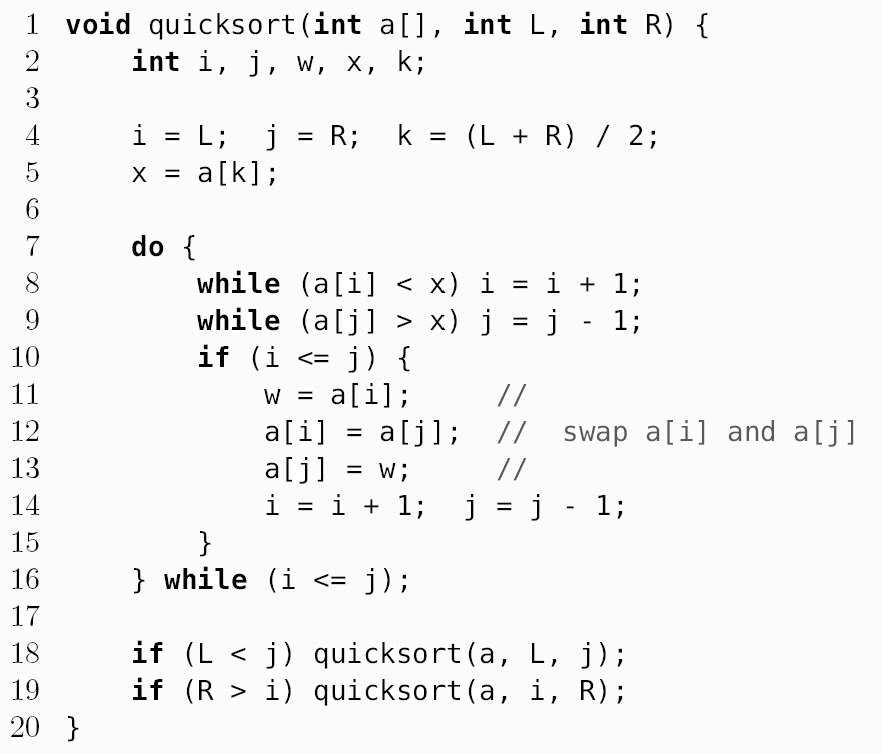
\includegraphics[height=.95\textheight]{./tut07_quicksort.jpg}
\end{frame}

\begin{frame} \frametitle{Aufgabe 1}
	\begin{columns}[t]
		\begin{column}{\dimexpr0.5\linewidth-\fboxrule-\fboxsep}
			\textbf{1. Durchlauf} \\[1em]
			\centering
			
			\begin{tabular}{ccccc}
				4 & 7 & \fbox{6} & 2 & 9 \\
				$\uparrow$ & & & & $\uparrow$ \\
				$i$ &&&& $j$ \\
				
				4 & 7 & \fbox{6} & 2 & 9 \\
				& $\uparrow$  && $\uparrow$ &\\
				& $i$ && $j$ & \\
				
				4 & 2 & \fbox{6} & 7 & 9 \\
				& & $\uparrow$ &&\\
				& & $i,j$ & & \\
				
				4 & 2 & \fbox{6} & 7 & 9 \\
				& $\uparrow$  && $\uparrow$ &\\
				& $j$ && $i$ & \\
			\end{tabular}
		\end{column}
		\begin{column}{\dimexpr0.5\linewidth-\fboxrule-\fboxsep}
			\textbf{2. Durchlauf} \\[1em]
			\centering
			
			\begin{tabular}{cc||c||cc}
				\fbox{4} & 2 & \fbox{6} & \fbox{7} & 9 \\
				$\uparrow$ & $\uparrow$ & & $\uparrow$ & $\uparrow$ \\
				$i$ & $j$ && $i$ & $j$ \\
				
				2 & \fbox{4} & \fbox{6} & \fbox{7} & 9 \\
				$\uparrow$ & $\uparrow$ & & $\uparrow$ & \\
				$j$ & $i$ && $i,j$ & \\
				
				2 & \fbox{4} & \fbox{6} & \fbox{7} & 9 \\
				&  & $\uparrow$ & & $\uparrow$  \\
				&  & $j$ & & $i$ \\
			\end{tabular}
		\end{column}
	\end{columns}
\end{frame}

%%%%%%%%%%%%%%%%%%%%%%%%%%%%%%%%%%%%%%%%%%%%%%%%%%%%%%%%%%%%%%%%%%%%%%%%%%%%%%%%%%%

\begin{frame} \frametitle{Binärbäume mit Heap-Eigenschaft}
	\small
	\begin{itemize}
		\item \textbf{Heap-Eigenschaft:}
		\begin{itemize}
			\item Für jeden Knoten $n$ gilt: Wenn $n$ mit $h$ beschriftet ist, dann müssen die Beschriftungen der Nachfolger von $n$ kleiner als $h$ sein (an der Wurzel eines Teilbaums stets stets der größte Schlüssel des Teilbaums) $\to$ \textit{Heap-Eigenschaft}
		\end{itemize}
		\item Herstellung der Heap-Eigenschaft: Funktion \textit{sinkenlassen}
		\begin{itemize}
			\item Sinkenlassen eines Knotens in Richtung Blätter
			\item Vertauschen von Wurzelbeschriftung mit größerem Kind
			\item Beispiel: $\qquad$ \fbox{\Tree [ .8 [ .9 ] [ .5 ] ]} $\overset{s(8)}{\longrightarrow}$ \fbox{\Tree [ .9 [ .8 ] [ .5 ]]}
		\end{itemize}
	\end{itemize}
\end{frame}

\begin{frame} \frametitle{Heapsort}
	\begin{itemize}
		\item Bäume sind nur Veranschaulichung
		\item Algorithmus arbeitet auf Listen
		\item zwei Phasen
		\begin{itemize}
			\item \textbf{1. Phase:} Einsortieren in den Heap und Herstellen der Heap-Eigenschaft
			\item \textbf{2. Phase:} Führe Sortierschritt wiederholt durch:
			\begin{itemize}
				\item Tausch von Wurzel und ''letztem`` Element (tiefste Ebene, ganz rechts)
				\item Fixiere dieses Element
				\item Sinkenlassen des neuen Wurzelelements
			\end{itemize}
		\end{itemize}
	\end{itemize}
\end{frame}

\begin{frame} \frametitle{Aufgabe 2 --- Phase 1}
	\begin{tabularx}{\linewidth}{m{.8cm} m{4cm}m{.8cm}m{4cm}}
		& \Tree [ .2 [ .0 [ .3  [ .1 ] [ .6 ]] [ .5 [ .7 ]  ] ] [ .9 [ .8 ] [ .4 ] ] ]
		&
		$\overset{s(3), s(5)}{\longrightarrow}$
		&
		\Tree [ .2 [ .0 [ .6  [ .1 ] [ .3 ]] [ .7 [ .5 ]  ] ] [ .9 [ .8 ] [ .4 ] ] ] \\
		$\overset{s(0), s(9)}{\longrightarrow}$
		&
		\Tree [ .2 [ .7 [ .6  [ .1 ] [ .3 ]] [ .5 [ .0 ]  ] ] [ .9 [ .8 ] [ .4 ] ] ]
		&
		$\overset{s(2)}{\longrightarrow}$
		&
		\Tree [ .9 [ .7 [ .6  [ .1 ] [ .3 ]] [ .5 [ .0 ]  ] ] [ .8 [ .2 ] [ .4 ] ] ]
	\end{tabularx}
\end{frame}

\begin{frame} \frametitle{Aufgabe 2 --- Phase 2}
	\begin{tabularx}{\linewidth}{m{.8cm}m{4cm}m{.8cm}m{4cm}}
		$\overset{\text{Tausch}}{\longrightarrow}$ 
		&
		\Tree [ .0 [ .7 [ .6  [ .1 ] [ .3 ]] [ .5 [ .\fbox{9} ]  ] ] [ .8 [ .2 ] [ .4 ] ] ] 
		&
		$\overset{s(0)}{\longrightarrow}$
		&
		\Tree [ .8 [ .7 [ .6  [ .1 ] [ .3 ]] [ .5 [ .\fbox{9} ]  ] ] [ .4 [ .2 ] [ .0 ] ] ] \\
		$\overset{\text{Tausch}}{\longrightarrow}$ 
		&
		\Tree [ .3 [ .7 [ .6  [ .1 ] [ .\fbox{8} ]] [ .5 [ .\fbox{9} ]  ] ] [ .4 [ .2 ] [ .0 ] ] ] 
		&
		$\overset{s(3)}{\longrightarrow}$
		&
		\Tree [ .7 [ .6 [ .3  [ .1 ] [ .\fbox{8} ]] [ .5 [ .\fbox{9} ]  ] ] [ .4 [ .2 ] [ .0 ] ] ] \\
	\end{tabularx}
\end{frame}

\begin{frame} \frametitle{Aufgabe 2 --- Phase 2}
	\textit{Fortsetzung zur Vollständigkeit}
	
	\begin{tabularx}{\linewidth}{m{.8cm}m{4cm}m{.8cm}m{4cm}}
		\onslide+<1->{$\overset{\text{Tausch}}{\longrightarrow}$}
		&
		\onslide+<1->{\Tree [ .1 [ .6 [ .3  [ .\fbox{7} ] [ .\fbox{8} ]] [ .5 [ .\fbox{9} ]  ] ] [ .4 [ .2 ] [ .0 ] ] ]}
		&
		\onslide+<2->{$\overset{s(1)}{\longrightarrow}$}
		&
		\onslide+<2->{\Tree [ .6 [ .5 [ .3  [ .\fbox{7} ] [ .\fbox{8} ]] [ .1 [ .\fbox{9} ]  ] ] [ .4 [ .2 ] [ .0 ] ] ]} \\
		\onslide+<3->{$\overset{\text{Tausch}}{\longrightarrow}$}
		&
		\onslide+<3->{\Tree [ .0 [ .5 [ .3  [ .\fbox{7} ] [ .\fbox{8} ]] [ .1 [ .\fbox{9} ]  ] ] [ .4 [ .2 ] [ .\fbox{6} ] ] ]}
		&
		\onslide+<4->{$\overset{s(0)}{\longrightarrow}$}
		&
		\onslide+<4->{\Tree [ .5 [ .3 [ .0  [ .\fbox{7} ] [ .\fbox{8} ]] [ .1 [ .\fbox{9} ]  ] ] [ .4 [ .2 ] [ .\fbox{6} ] ] ] } \\
	\end{tabularx}
\end{frame}

\begin{frame} \frametitle{Aufgabe 2}
	\textit{Fortsetzung zur Vollständigkeit}
	
	\begin{tabularx}{\linewidth}{m{.8cm}m{4cm}m{.8cm}m{4cm}}
		\onslide+<1->{$\overset{\text{Tausch}}{\longrightarrow}$} 
		&
		\onslide+<1->{\Tree [ .2 [ .3 [ .0  [ .\fbox{7} ] [ .\fbox{8} ]] [ .1 [ .\fbox{9} ]  ] ] [ .4 [ .\fbox{5} ] [ .\fbox{6} ] ] ] }
		&
		\onslide+<2->{$\overset{s(2)}{\longrightarrow}$} 
		&
		\onslide+<2->{\Tree [ .4 [ .3 [ .0  [ .\fbox{7} ] [ .\fbox{8} ]] [ .1 [ .\fbox{9} ]  ] ] [ .2 [ .\fbox{5} ] [ .\fbox{6} ] ] ] } \\
		\onslide+<3->{$\overset{\text{Tausch}}{\longrightarrow}$}
		&
		\onslide+<3->{\Tree [ .1 [ .3 [ .0  [ .\fbox{7} ] [ .\fbox{8} ]] [ .\fbox{4} [ .\fbox{9} ]  ] ] [ .2 [ .\fbox{5} ] [ .\fbox{6} ] ] ] }
		&
		\onslide+<4->{$\overset{s(1)}{\longrightarrow}$ }
		&
		\onslide+<4->{\Tree [ .3 [ .1 [ .0  [ .\fbox{7} ] [ .\fbox{8} ]] [ .\fbox{4} [ .\fbox{9} ]  ] ] [ .2 [ .\fbox{5} ] [ .\fbox{6} ] ] ] } \\
	\end{tabularx}
\end{frame}

\begin{frame} \frametitle{Aufgabe 2}
	\textit{Fortsetzung zur Vollständigkeit}
	
	\begin{tabularx}{\linewidth}{m{.8cm}m{4cm}m{.8cm}m{4cm}}
		\onslide+<1->{$\overset{\text{Tausch}}{\longrightarrow}$ }
		&
		\onslide+<1->{\Tree [ .0 [ .1 [ .\fbox{3}  [ .\fbox{7} ] [ .\fbox{8} ]] [ .\fbox{4} [ .\fbox{9} ]  ] ] [ .2 [ .\fbox{5} ] [ .\fbox{6} ] ] ] }
		&
		\onslide+<2->{$\overset{s(0)}{\longrightarrow}$} 
		&
		\onslide+<2->{\Tree [ .2 [ .1 [ .\fbox{3}  [ .\fbox{7} ] [ .\fbox{8} ]] [ .\fbox{4} [ .\fbox{9} ]  ] ] [ .0 [ .\fbox{5} ] [ .\fbox{6} ] ] ] } \\
		%
		\onslide+<3->{$\overset{\text{Tausch}}{\longrightarrow}$ }
		&
		\onslide+<3->{\Tree [ .0 [ .1 [ .\fbox{3}  [ .\fbox{7} ] [ .\fbox{8} ]] [ .\fbox{4} [ .\fbox{9} ]  ] ] [ .\fbox{2} [ .\fbox{5} ] [ .\fbox{6} ] ] ] }
		&
		\onslide+<4->{$\overset{s(0)}{\longrightarrow}$ }
		&
		\onslide+<4->{\Tree [ .1 [ .0 [ .\fbox{3}  [ .\fbox{7} ] [ .\fbox{8} ]] [ .\fbox{4} [ .\fbox{9} ]  ] ] [ .\fbox{2} [ .\fbox{5} ] [ .\fbox{6} ] ] ] } \\
	\end{tabularx}
\end{frame}

\begin{frame} \frametitle{Aufgabe 2}
	\textit{Fortsetzung zur Vollständigkeit}
	
	\begin{tabularx}{\linewidth}{m{.8cm}m{4cm}m{.8cm}m{4cm}}
		\onslide+<1->{$\overset{\text{Tausch}}{\longrightarrow}$ }
		&
		\onslide+<1->{\Tree [ .0 [ .1 [ .\fbox{3}  [ .\fbox{7} ] [ .\fbox{8} ]] [ .\fbox{4} [ .\fbox{9} ]  ] ] [ .\fbox{2} [ .\fbox{5} ] [ .\fbox{6} ] ] ]}
		&
		\onslide+<2->{$\overset{s(0)}{\longrightarrow}$ }
		&
		\onslide+<2->{\Tree [ .1 [ .0 [ .\fbox{3}  [ .\fbox{7} ] [ .\fbox{8} ]] [ .\fbox{4} [ .\fbox{9} ]  ] ] [ .\fbox{2} [ .\fbox{5} ] [ .\fbox{6} ] ] ] } \\
		\onslide+<3->{$\overset{\text{Tausch}}{\longrightarrow}$ }
		&
		\onslide+<3->{\Tree [ .0 [ .\fbox{1} [ .\fbox{3}  [ .\fbox{7} ] [ .\fbox{8} ]] [ .\fbox{4} [ .\fbox{9} ]  ] ] [ .\fbox{2} [ .\fbox{5} ] [ .\fbox{6} ] ] ]}
		&
		\onslide+<4->{$\overset{}{\longrightarrow}$ }
		&
		\onslide+<4->{\Tree [ .\fbox{0} [ .\fbox{1} [ .\fbox{3}  [ .\fbox{7} ] [ .\fbox{8} ]] [ .\fbox{4} [ .\fbox{9} ]  ] ] [ .\fbox{2} [ .\fbox{5} ] [ .\fbox{6} ] ] ]}
	\end{tabularx}
\end{frame}

\begin{frame} \frametitle{Aufgabe 2}
	\centering 
	sortierte Liste: \\
	\texttt{[ 0, 1, 2, 3, 4, 5, 6, 7, 8, 9 ]} \\
	\vspace{1cm}
	\textbf{FERTIG \smiley}
\end{frame}

%%%%%%%%%%%%%%%%%%%%%%%%%%%%%%%%%%%%%%%%%%%%%%%%%%%%%%%%%%%%%%%%%%%%%%%%%%%%%%%%%%%


%%%%%%%%%%%%%%%%%%%%%%%%%%%%%%%%%%%%%%%%%%%%%%%%%%%%%%%%%%%%%%%%%%%%%%%%%%%%%%%%%%%





%%%%%%%%%%%%%%%%%%%%%%%%%%%%%%%%%%%%%%%%%%%%%%%%%%%%%%%%%%%%%%%%%%%%%%%%%%%%%%%%%%%

\end{document}